
%\documentclass[calculator,datasheet,solutions,resit]{exam} 
\documentclass[calculator,datasheet,resit]{exam}

% The full list of class options are
% calculator : Allows approved calculator use.
% datasheet : Adds a note that data sheet are attached to the exam.
% handbook : Allows the use of the engineering handbook.
% resit : Adds the resit markings to the paper.
% sample : Adds conspicuous SAMPLE markings to the paper
% solutions : Uses the contents of \solution commands (and \solmarks) to generate a solution file

\usepackage{pdfpages}
\usepackage{lscape,comment}

\coursecode{EG5597}%%
\coursetitle{Advanced Chemical Engineering}%

\examtime{00.00--00.00}%
\examdate{00}{06}{2015}%
\examformat{Candidates must attempt \textit{all} questions.}

\newcommand{\frc}{\displaystyle\frac}
\newcommand{\br}[1]{\!\left( #1 \right)}
\newcommand{\abs}[1]{\left| #1 \right|}
\newcommand{\fracd}[2]{\frac{\mathrm{d} #1}{\mathrm{d} #2}}
\newcommand{\fracp}[2]{\frac{\partial #1}{\partial #2}}
\renewcommand{\d}[1]{\mathrm{d} #1 }
\newcommand{\Ma}{\mathrm{M\!a}}



\begin{document}

%%%
%%% QUESTION
%%%
\begin{question}
\begin{enumerate}[(a)]

\item The Rankine cycle is used to convert thermal energy into power. Sketch a Rankine cycle as a pressure enthalpy chart. Describe the cycle.~\marks{8}

\item Given the following information and Mollier chart for the Organic Rankine fluid i-Pentane, estimate the amount of power in kW that could be recovered using a Rankine cycle with an electrical generator coupled to a turbine/expander. The source of heat for the cycle is hot water.
\begin{enumerate}[(i)]
\item Hot water volume  flow = 0.184 m$^{3}$/s
\item Hot water inlet temperature = 95$^{\circ}$C
\item Hot water outlet temperature = 75$^{\circ}$C
\item Hot Water density = 1000 kg/m$^{3}$
\item Hot water specific heat = 4.2 kJ/(kg.$^{\circ}$C)
\end{enumerate}
Assume i-Pentane enters the pump as a saturated liquid at 100 kPa, the pump operates isentropically and the discharge pressure is 350 kPa. Assume the turbine/expander inlet is a saturated vapour. Also, assume the turbine/expander isentropic efficiency is 75$\%$ and the electrical generator efficiency is 90$\%$. State any other assumptions.~\marks{12}
\begin{center}
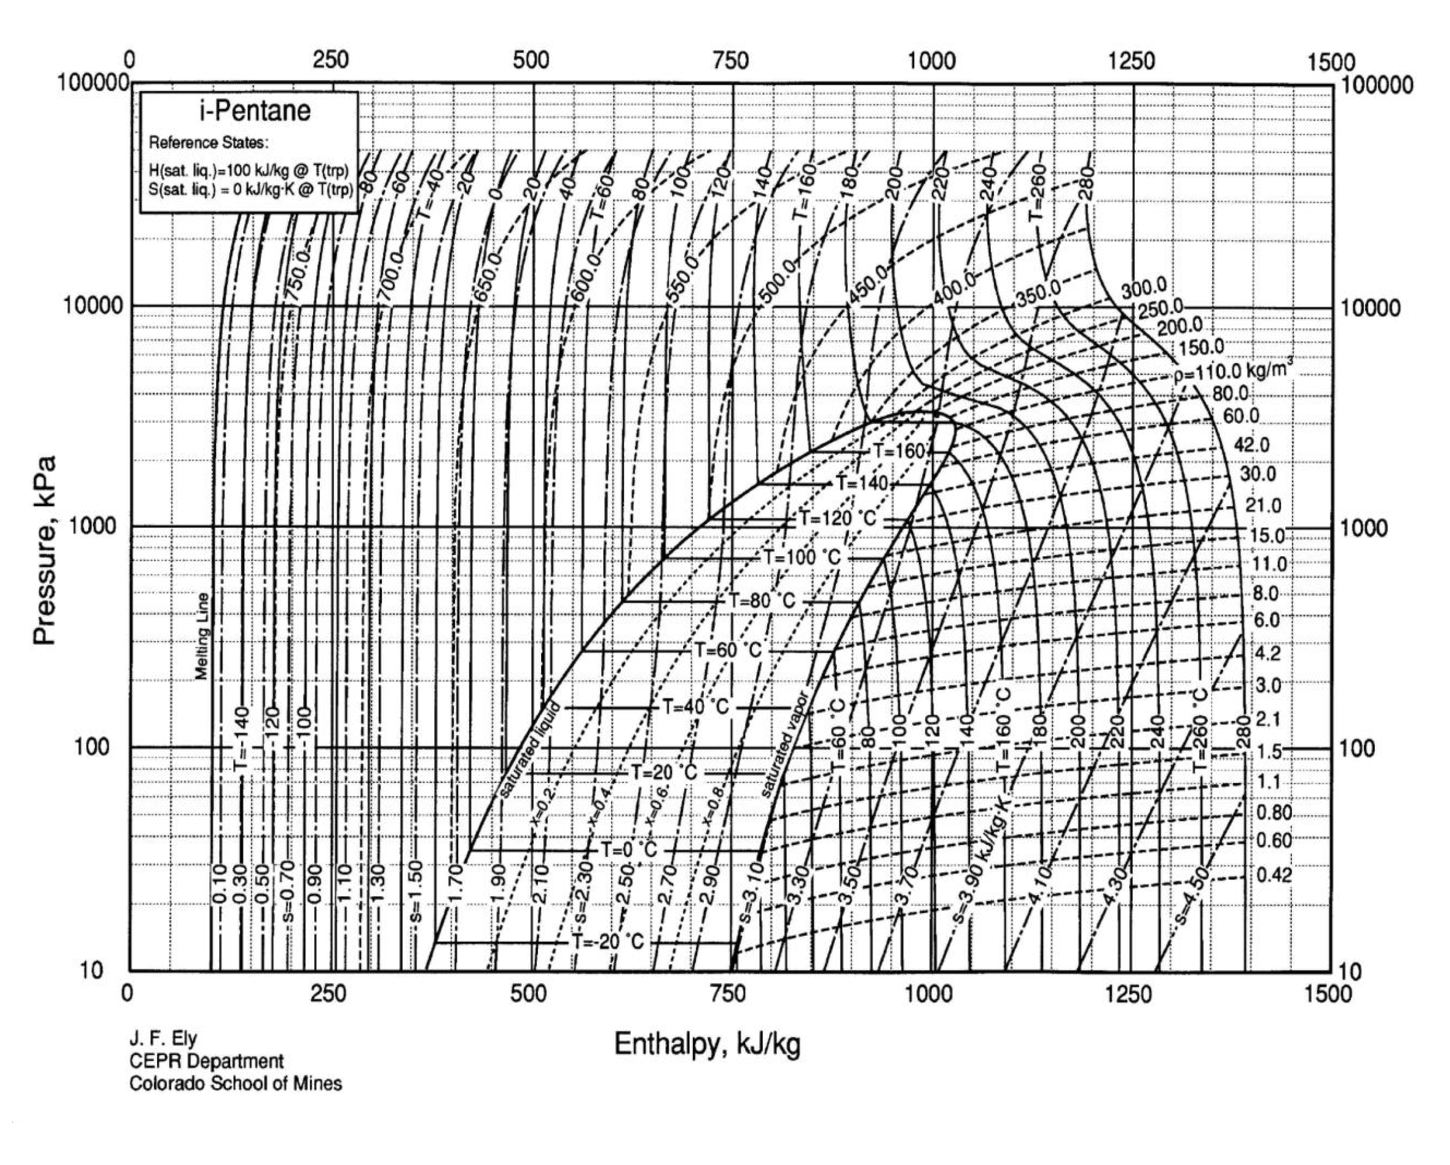
\includegraphics[width=\columnwidth]{./Pics/EG5597_Process_3_June_2014-5.pdf}
\end{center} 


\end{enumerate}
\end{question}

\clearpage

%%% 
%%% QUESTION
%%%
\begin{question}
\begin{enumerate}[(a)]
%
\item An oilfield with a 20 year life has the following energy demand:
\begin{center}
\begin{tabular}{c c |c c |c c |c c}
\hline
{\bf Year} & {\bf Load} & {\bf Year} & {\bf Load} & {\bf Year} & {\bf Load} & {\bf Year} & {\bf Load} \\
           & {\bf MW}   &            &   {\bf MW} &            &  {\bf MW}  &            &   {\bf MW} \\
\hline
1          & 22         & 6          & 24         & 11         & 24         & 16         & 24 \\
2          & 22         & 7          & 24         & 12         & 24         & 17         & 24 \\
3          & 22         & 8          & 26         & 13         & 24         & 18         & 24 \\
4          & 24         & 9          & 28         & 14         & 24         & 19         & 24 \\
5          & 24         & 10         & 28         & 15         & 24         & 20         & 24 \\
\hline
\end{tabular}
\end{center}
The choice of Gas Turbine to provide this power is between Solar Titan and a Solar Mars. Data for these two machines is as follows:
\begin{center}
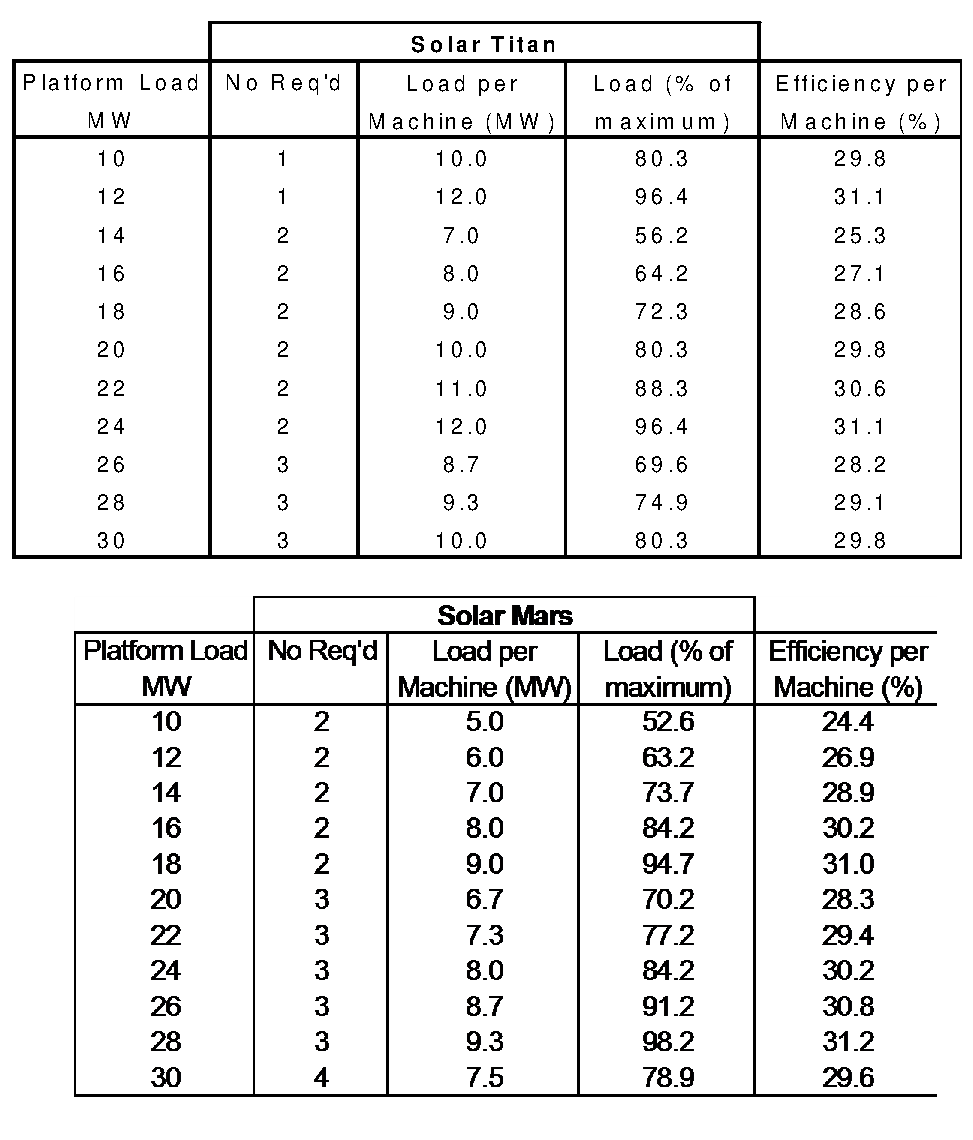
\includegraphics[width=0.8\columnwidth]{./Pics/EG5597_Process_4_June_2014-5.pdf} 
\end{center} 
By conducting an annual review of machine efficiencies and CO$_{2}$ production determine which GT would minimise CO$_{2}$ emissions over the field life.~\marks{12}

\item In order to reduce flaring rates an installation is considering deploying a Flare Gas Recovery System. Sketch and describe the key components of a flare gas recovery system.~\marks{8}


%
\end{enumerate}

\end{question}

\clearpage

%%% 
%%% QUESTION 
%%%
\begin{question}
Answer all of the following questions.

\begin{enumerate}[(a)]
\item Consider the closed-loop block diagram of the process given below, where $K_{p} > 0$, $\tau_{a} > 0$, and $\tau_{b} > 0$. Investigate the stability of the system applying the Routh-Hurwitz stability criterion.~\marks{8}
\begin{center}
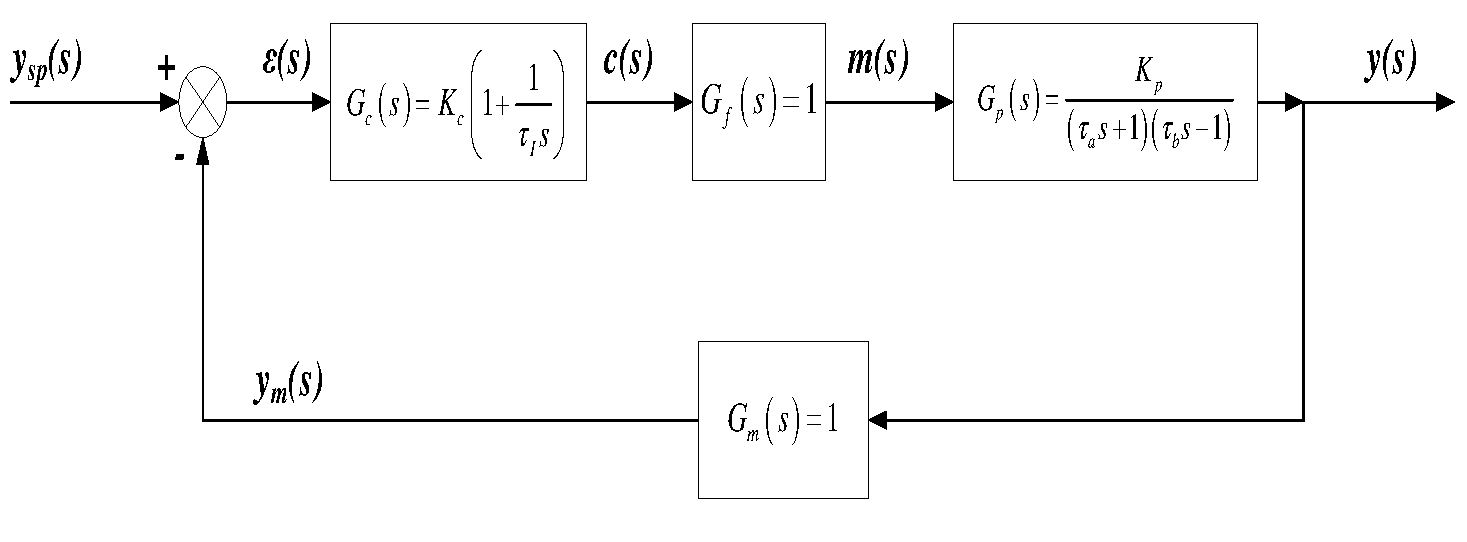
\includegraphics[width=\columnwidth]{./Pics/EG5597_Control_1_June_2014-5.pdf}
\end{center} 

\item Applying the 7 rules for Root-Locus definition, construct the Root-Locus of the closed-loop control system given below. If the Root-Locus crosses the {\it Im}-axis, apply the Routh-Hurwitz stability criterion to find the exact points of intersection. The Root-Locus should be qualitative, but correct on all structural features.~\marks{12}
\begin{center}
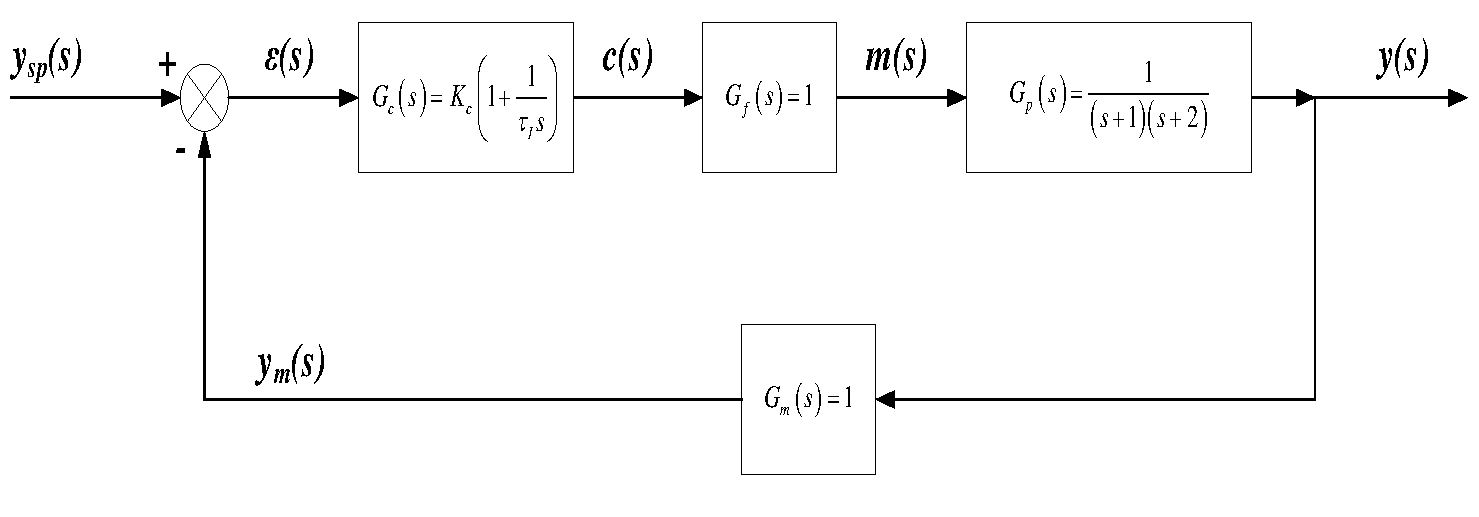
\includegraphics[width=\columnwidth]{./Pics/EG5597_Control_2_June_2014-5.pdf}
\end{center} 
wher $\tau_{I}=0.25$.

\end{enumerate}




\underline{Useful equations}: 
\begin{itemize}
\item Asymptotes angles with positive direction of {\it Re}-axis: 
\begin{displaymath}
\varphi_{i} = \frc{2k + 1}{n -m}\pi,\;\;\;k=0,\cdots,n-m-1
\end{displaymath}

\item Asymptotes centre of gravity:
\begin{displaymath}
\gamma=\frc{\left[\sum\limits_{i=1}^{n}p_{i}-\sum\limits_{j=1}^{m}z_{i}\right]}{(n-m)}
\end{displaymath}

\item Departure/arrival points of branches: 
\begin{displaymath}
\sum\limits_{i=1}^{n}\frc{1}{\left(s_{0}-p_{i}\right)}=\sum\limits_{j=1}^{m}\frc{1}{\left(s_{0}-z_{j}\right)}
\end{displaymath} 
\end{itemize}


\end{question}


\clearpage


%%%%%%%%%%%%%%%%%%%%%%%%%
%%% Question 04       %%%
%%%%%%%%%%%%%%%%%%%%%%%%%
\begin{question} 
A new F1-car front-wing air-foil needs to be designed. The back part of the air-foil is in contact with the car nose (chassis) and the outer part is in contact with flowing air. The temperature of chassis is 200$^{\circ}$C and the ambient air temperature is 20$^{\circ}$C. Heat loss in the tip of the air-foil is assumed negligible. Air is assumed as incompressible, car nose and air temperatures are constant. The temperature across the air-foil can be expressed as an 1-D elliptic partial differential equation,
\begin{displaymath}
\frc{\partial^{2} T}{\partial x^{2}} -\alpha T = -\alpha T_{\text{amb}}
\end{displaymath} 
where $\alpha=20\;^{\text{o}}$C.m$^{-2}$ and $T_{\text{amb}}$ is the temperature of the flowing air. Estimate the temperature profile at 4 nodes equally spaced in the air-foil of length $L=0.30$m. The central-difference scheme for the second-order derivative is,~\marks{20}
\begin{displaymath}
\frc{\partial^{2} T}{\partial x^{2}} = \frc{T_{i+1}-2T_{i}+T_{i-1}}{\left(\Delta x\right)^{2}}
\end{displaymath}
\end{question}
 


\clearpage

%%%%%%%%%%%%%%%%%%%%%%%%%
%%% Question 05       %%%
%%%%%%%%%%%%%%%%%%%%%%%%%
\begin{question}
\begin{enumerate}[(a)]
\item A particular case of PDE's is
\begin{displaymath}
u_{t}+\alpha u_{x} = \kappa u_{xx}
\end{displaymath}
that represents advection-diffusion problems (with constant coefficients $\alpha$ and $\kappa$) with a number of applications in fluid and solid mechanics. Demonstrate that the advection term (in 1D and assuming regular grid) is
\begin{displaymath}
\frc{\partial u}{\partial x}=\frc{u_{i+1}-u_{i}}{\Delta x_{i}} + \mathcal{O}\left(\Delta x\right)
\end{displaymath}
using Taylor's expansion.
\end{enumerate}
\end{question}


\vfill


\paperend

\end{document}
